%%%%%%%%%%%%%%%%%%%%%%%%%%%%%%%%%%%%%%%%%%%%%%%%%%%%%%%%%%%%%%%
%
%
%%%%%%%%%%%%%%%%%%%%%%%%%%%%%%%%%%%%%%%%%%%%%%%%%%%%%%%%%%%%%%%

\documentclass{article}
\usepackage{graphicx}
\usepackage{fullpage}
\usepackage{amsmath}

\title{Übungsblatt 4}
\author{Tobias Baake (247074), Dylan Ellinger (247316), Nikiforos Tompoulidis (247714)}
\begin{document}
\maketitle

\section{Aufgabe Bernstein-Polynome}
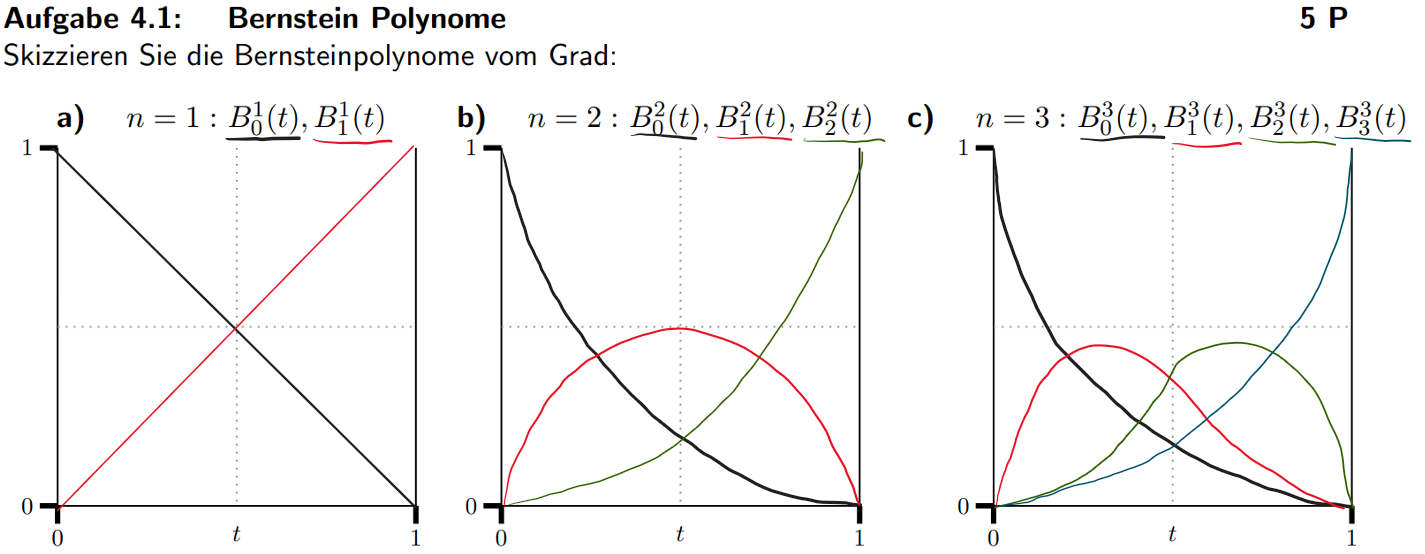
\includegraphics[width=400pt]{./files/Übung4.1.png}

\section{Aufgabe B-Spline Basisifunktion}
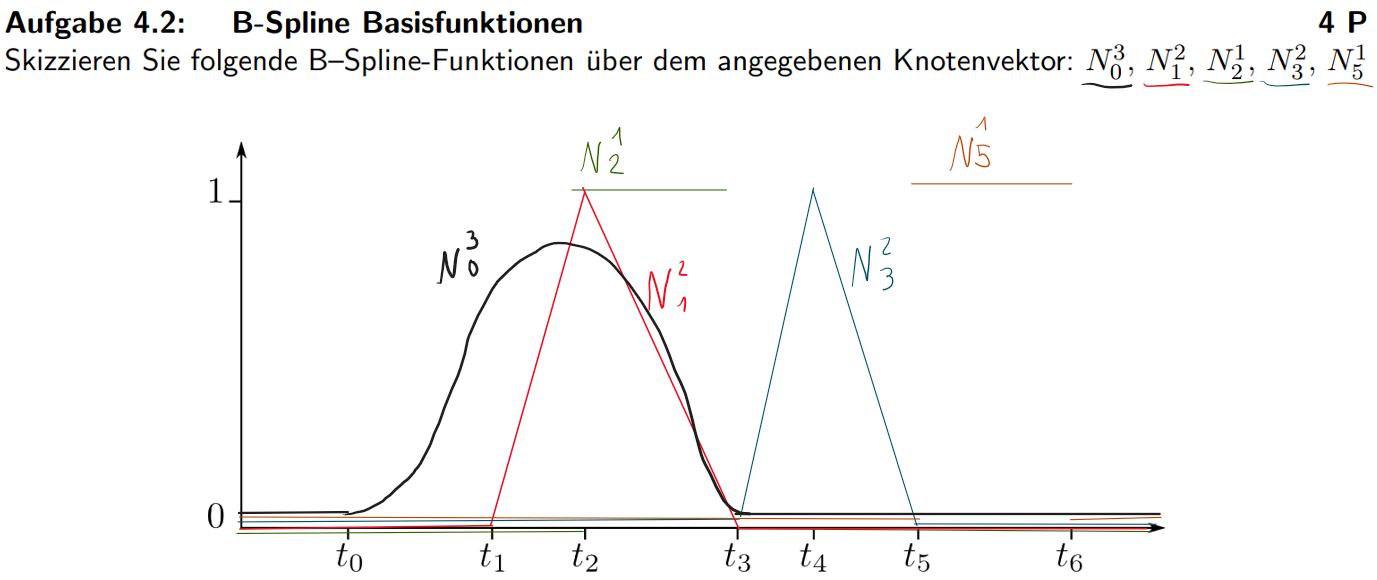
\includegraphics[width=400pt]{./files/Übung4.2.png}
\\
\\
\\
\section{Aufgabe Tensorproduktflächen}

\emph{a)}\\
$x(1,0) = b_{0,0} B_0^1(1) + + b_{1,0} B_1^1(1) B_0^1(0) + b_{0,1} B_0^1(1) B_1^1(0) + b_{1,1} B_1^1(1) B_1^1(0) $ \\
\\ mit $( B_0^1(1) = 1 )$ und $( B_1^1(1) = 0 )$ \\
$x(1,0) = b_{0,0} + 0 + 0 + 0 = \underline{b_{0,0}}$ \\
\\
\emph{b)}\\
$ x(0.5, 0.5) = b_{0,0} B_0^1(0.5) B_0^1(0.5) + b_{1,0} B_1^1(0.5) B_0^1(0.5) + b_{0,1} B_0^1(0.5) B_1^1(0.5) + b_{1,1} B_1^1(0.5) B_1^1(0.5) $ \\
\\ mit $( B_0^1(0.5) = 0.5 )$ und $( B_1^1(0.5) = 0.5 )$ \\
$ x(0.5, 0.5) = \underline{0.25 b_{0,0} + 0.25 b_{1,0} + 0.25 b_{0,1} + 0.25 b_{1,1}} $ \\
\\
\emph{c)}\\
$ x\left(\frac{2}{5}, \frac{1}{3}\right) = b_{0,0} B_0^1\left(\frac{2}{5}\right) B_0^1\left(\frac{1}{3}\right) + b_{1,0} B_1^1\left(\frac{2}{5}\right) B_0^1\left(\frac{1}{3}\right) + b_{0,1} B_0^1\left(\frac{2}{5}\right) B_1^1\left(\frac{1}{3}\right) + b_{1,1} B_1^1\left(\frac{2}{5}\right) B_1^1\left(\frac{1}{3}\right) $ \\
\\ mit $( B_0^1\left(\frac{2}{5}\right) = \frac{3}{5} )$, $( B_1^1\left(\frac{2}{5}\right) = \frac{2}{5} )$, $( B_0^1\left(\frac{1}{3}\right) = \frac{2}{3} )$ und $( B_1^1\left(\frac{1}{3}\right) = \frac{1}{3} )$ \\
$ x\left(\frac{2}{5}, \frac{1}{3}\right) = \underline{\frac{3}{25} b_{0,0} + \frac{4}{25} b_{1,0} + \frac{2}{25} b_{0,1} + \frac{1}{25} b_{1,1}} $\\
\\

\section{Aufgabe Kreisbogen}
Um zu beweisen, dass die gegebene rationale Bézierkurve $ r(t) $ ein Viertel des Einheitskreises ist, müssen wir die Punkte auf der Kurve betrachten.\\
\\
Ein Punkt auf einem Kreis mit Radius 1 (Einheitskreis) muss die Gleichung $ x^2 + y^2 = 1 $ erfüllen.\\
Da wir einen Viertel des Einheitskreises betrachten müssen wir prüfen, dass die Punkte nur im ersten Quadranten des Koordinatensystems liegen (\( x \geq 0 \) und \( y \geq 0 \)).\\
\\
geg. Kurve: $ r(t) $:\\
$ r(t) = (1-t)^2 \cdot b_0 + 2(1-t)t \cdot b_1 + t^2 \cdot b_2 $\\
\\
mit den Kontrollpunkten $ b_0 = (1, 0) $, $ b_1 = (1, 1) $, $ b_2 = (0, 1) $ und den Gewichten $ w_0 = 1 $, $ w_1 = \sqrt{2}/2 $, $ w_2 = 1 $ im Intervall $ t \in [0, 1] $.
\\
\\
Einsetzen:\\
\\
\begin{align*}
r(t) &= (1-t)^2 \cdot (1, 0) + 2(1-t)t \cdot (1, 1) + t^2 \cdot (0, 1) \\
&= ((1-t)^2, 0) + 2(1-t)t \cdot (1, 1) + (0, t^2) \\
&= ((1-t)^2 + 2(1-t)t, 2(1-t)t + t^2) \\
&= ((1 - 2t + t^2) + 2(t - 2t^2), 2t - 2t^2 + t^2) \\
&= (1 - 2t + t^2 + 2t - 4t^2, 2t - 2t^2 + t^2) \\
&= (1 - 2t + 2t - 4t^2, 2t - 2t^2 + t^2) \\
&= (1 - 4t^2, 2t - t^2)
\end{align*}
\\
Einsetzen der Bézierkurve in die Gleichung vom Einheitskreis $ x^2 + y^2 = 1 $:\\
\\
$ (1 - 4t^2)^2 + (2t - t^2)^2 = 1 $\\
$ 17t^4 - 4t^3 - 4t^2 + 0 = 0 $\\
$ 17t^4 - 4t^3 - 4t^2 = 0$\\
\\
Lsg:\\ $ t = 0 $, $ t = 1 $, $ t = \frac{2}{17}(1 + \sqrt{3}) $ und $ t = \frac{2}{17}(1 - \sqrt{3}) $\\
Aufgrund des Intervalls betrachten wir nur die Lösungen \( t = 0 \) und \( t = 1 \).\\
\\
Wenn \( t = 0 \), dann ist \( r(t) = (1, 0) \), was auf dem Einheitskreis liegt.\\
Wenn \( t = 1 \), dann ist \( r(t) = (0, 1) \), was ebenfalls auf dem Einheitskreis liegt.\\
\\
$\Rightarrow$ Somit liegen die Endpunkte der Bézierkurve auf dem Einheitskreis.
\end{document}

